\documentclass[tikz,border=14pt]{standalone}
\usepackage{tikz}
\usepackage{amsmath}
\usetikzlibrary{arrows.meta,calc,positioning}

\begin{document}
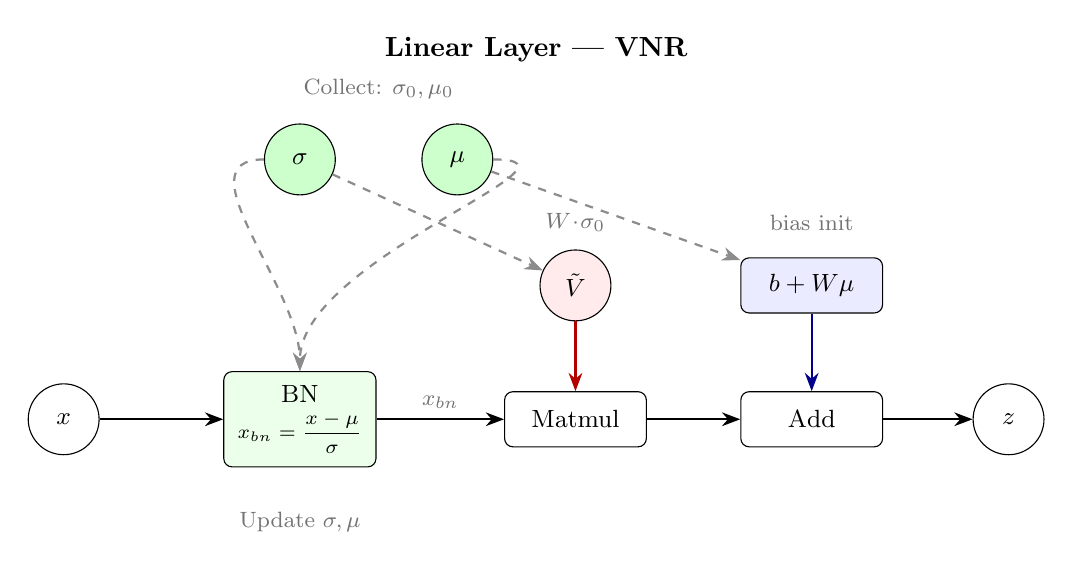
\begin{tikzpicture}[
  >=Stealth,
  box/.style={draw, rounded corners=3pt, minimum width=1.8cm, minimum height=0.7cm,
              inner sep=5pt, font=\small, align=center},
  param/.style={draw, circle, minimum size=0.9cm, inner sep=1pt, font=\small},
  annot/.style={font=\footnotesize, text=black!55},
  arr/.style={->, thick},
  radd/.style={->, red!70!black, thick},
  badd/.style={->, blue!55!black, thick},
  darrw/.style={->, dashed, black!45, thick},
]

%% ═══ LINEAR ═══════════════════════════════════════════════════════════
\node[font=\normalsize\bfseries] at (6.0, 5.2) {Linear Layer — VNR};

% BN statistics at the top
\node[param, fill=green!20] (lsigma) at (3.0, 3.8) {$\sigma$};
\node[param, fill=green!20] (lmu)    at (5.0, 3.8) {$\mu$};
\node[annot] at (4.0, 4.7) {Collect: $\sigma_0, \mu_0$};

% Main forward pass
\node[param]             (lx)   at (0,   0.5) {$x$};
\node[box, fill=green!8] (lbn)  at (3.0, 0.5)
    {BN\\[2pt]\scriptsize$x_{bn}=\dfrac{x-\mu}{\sigma}$};
\node[annot]             at (3.0, -0.8) {Update $\sigma,\mu$};
\node[box]               (lmul) at (6.5, 0.5) {Matmul};
\node[box]               (ladd) at (9.5, 0.5) {Add};
\node[param]             (lz)   at (12.0, 0.5) {$z$};

% Parameters for Matmul (red) - initialized with σ
\node[param, fill=red!8]  (lvt) at (6.5,  2.2) {$\tilde{V}$};
\node[annot] at (6.5,  3.0) {$W\!\cdot\!\sigma_0$};

% Parameters for Add (blue) - initialized with μ
\node[box, fill=blue!8]   (lbias) at (9.5, 2.2) {$b + W\mu$};
\node[annot] at (9.5,  3.0) {bias init};

% Main forward arrows
\draw[arr]  (lx)  -- (lbn);
\draw[arr]  (lbn) -- node[above, annot]{$x_{bn}$} (lmul);
\draw[arr]  (lmul)-- (ladd);
\draw[arr]  (ladd)-- (lz);
\draw[radd] (lvt) -- (lmul);
\draw[badd] (lbias) -- (ladd);

% σ flows from top to V̂
\draw[darrw] (lsigma) -- (lvt);

% μ flows from top to bias box
\draw[darrw] (lmu) -- (lbias);

% Statistics update from BN
\draw[darrw, in=90, out=180] (lsigma) to (lbn);
\draw[darrw, in=90, out=0] (lmu) to (lbn);

\end{tikzpicture}
\end{document}
